\documentclass[letterpaper,11pt]{amsart}

\usepackage{amscd,amssymb,amsfonts,amsmath,amsthm,color}
\usepackage{enumerate}
\usepackage{listings}
\usepackage{courier}
\usepackage{graphicx}
\usepackage{scrextend}

\usepackage{calc}
\newsavebox\CBox
\newcommand\hcancel[2][0.5pt]{%
  \ifmmode\sbox\CBox{$#2$}\else\sbox\CBox{#2}\fi%
  \makebox[0pt][l]{\usebox\CBox}%  
  \rule[0.5\ht\CBox-#1/2]{\wd\CBox}{#1}}


\lstset{frame=lrbt,xleftmargin=\fboxsep,xrightmargin=-\fboxsep,colframe=gray}


\lstset{basicstyle=\ttfamily\footnotesize,breaklines=true}


%%%%%%%%%%%%%%%%%%%%%%%%%%%%%%%%%%%%%%%%%%%%%%%%%%%%%%%%%%%%
% margins and style
\pagestyle{plain}
\setlength{\evensidemargin}{0.25in}
\setlength{\oddsidemargin}{0.25in}
\setlength{\textwidth}{6.0in}
\setlength{\topmargin}{0.0in}
\setlength{\textheight}{8.5in}
\setlength{\headheight}{0in}
\setlength{\parskip}{1.5mm}

\linespread{1.2}
\usepackage{color}
\definecolor{gray}{rgb}{0.3,0.3,0.3}



%%%%%%%%%%%%%%%%%%%%%%%%%%%%%%%%%%%%%%%%%%%%%%%%%%%%%%%%%%%%
% theorems and all 
\theoremstyle{plain}
\newtheorem{theorem}{Theorem}[section]
\newtheorem{lemma}[theorem]{Lemma}
\newtheorem{proposition}[theorem]{Proposition}
\newtheorem{corollary}[theorem]{Corollary}

\theoremstyle{definition}
\newtheorem{definition}[theorem]{Definition}
\newtheorem{remark}[theorem]{Remark}

%%%%%%%%%%%%%%%%%%%%%%%%%%%%%%%%%%%%%%%%%%%%%%%%%%%%%%%%%%%%
% renewed commands: t, to, d , c, H

%%%%%%%%%%%%%%%%%%%%%%%%%%%%%%%%%%%%%%%%%%%%%%%%%%%%%%%%%%%%
% Shortcuts for tex commands

\newcommand{\nc}{\newcommand}
\newcommand{\rc}{\renewcommand}
\nc{\mc}{\mathcal}
\rc{\t}{\text}
\nc{\loccit}{\emph{loc. cit. }}
\nc\pf{\noindent Proof: }
%%%%%%%%%%%%%%%%%%%%%%%%%%%%%%%%%%%%%%%%%%%%%%%%%%%%%%%%%%%%
% Operators, functions etc
\nc{\Hom}{\t{Hom}}
\nc{\tot}{\t{tot}}
\nc{\dual}{^{\vee}}
\nc{\op}[1]{\operatorname{#1}}
\nc{\coh}{\t{coh}}
\nc{\iso}{\cong}
\rc{\d}{\operatorname{d}}
\nc{\Id}{\operatorname{Id}}
\nc{\dgmod}{\operatorname{dg-mod}}
\newcommand{\hdot}{^{\raisebox{0pt}{\text{\circle*{2}}}}}
\nc{\compose}{\circ}
\nc{\sheafsym}{\mathcal{S}\t{ym}}
\nc{\rend}{\operatorname{REnd}}
\nc{\rhom}{\operatorname{RHom}}
\nc{\sheafrend}{\mathcal{R}\mc{E}\t{\emph{nd}}}
\nc{\sheafrhom}{\mathcal{R}\mc{H}\t{\emph{om}}}
\nc{\sheafhom}{\mathcal{H}\t{om}}
\nc{\exterior}{{\textstyle\bigwedge\nolimits}}
\nc{\ex}{\exterior}
\nc{\cok}{\operatorname{Coker}}
\rc{\ker}{\operatorname{Ker}}
\nc{\im}{\operatorname{Im}}

%tensor product
\nc{\Lotimes}{{\overset{L}{\otimes}}}
%%%%%%%%%%%%%%%%%%%%%%%%%%%%%%%%%%%%%%%%%%%%%%%%%%%%%%%%%%%%
% Arrows and signs
\rc{\to}{\rightarrow}
\nc{\ot}{\leftarrow}
\nc\xto[1]{\xrightarrow{#1}}
\nc{\too}{\longrightarrow}
\nc{\oot}{\longleftarrow}
\nc{\into}{\hookrightarrow}
\nc{\mapsinto}{\hookrightarrow}
%%%%%%%%%%%%%%%%%%%%%%%%%%%%%%%%%%%%%%%%%%%%%%%%%%%%%%%%%%%%
% Categories
\nc{\D}{\operatorname{D}}
\nc{\Dsg}{\D_{{sg}}}
\nc{\Db}{\D^{{b}}}
\nc{\Dbgr}{\Db_{{gr}}}
\nc{\Dgr}{\D_{{gr}}}
\nc{\Dsggr}{\Dsg^{{gr}}}
\nc{\Cgr}{\operatorname{C}_{{gr}}}
\nc{\cCgr}{\cC_{gr}}
\nc{\cDgr}{\cD_{gr}}
\nc{\cDsggr}{\cD_{gr}^{sg}}
\nc{\cDbgr}{\cD_{gr}^{b}}
\nc{\cDsg}{\cD_{sg}}
\nc{\cDb}{\cD^{b}}
\rc{\H}{\operatorname{H}}

%%%%%%%%%%%%%%%%%%%%%%%%%%%%%%%%%%%%%%%%%%%%%%%%%%%%%%%%%%%%
% Nice letters
% cals
\nc{\cA}{\mc{A}}\nc{\cB}{\mc{B}}\nc{\cC}{\mc{C}}\nc{\cD}{\mc{D}}\nc{\cE}{\mc{E}}\nc{\cF}{\mc{F}}\nc{\cG}{\mc{G}}\nc{\cH}{\mc{H}}\nc{\cI}{\mc{I}}\nc{\cJ}{\mc{J}}\nc{\cK}{\mc{K}}\nc{\cL}{\mc{L}}\nc{\cM}{\mc{M}}\nc{\cN}{\mc{N}}\nc{\cO}{\mc{O}}\nc{\cP}{\mc{P}}\nc{\cQ}{\mc{Q}}\nc{\cR}{\mc{R}}\nc{\cS}{\mc{S}}\nc{\cT}{\mc{T}}\nc{\cU}{\mc{U}}\nc{\cV}{\mc{V}}\nc{\cW}{\mc{W}}\nc{\cX}{\mc{X}}\nc{\cY}{\mc{Y}}\nc{\cZ}{\mc{Z}}
% bbs
\nc{\PP}{\mathbb{P}}
\nc{\CC}{\mathbb{C}}
\nc{\ZZ}{\mathbb{Z}}
\nc{\HH}{\mathbb{H}}
\nc{\NN}{\mathbb{N}}
\nc{\QQ}{\mathbb{Q}}
\nc{\RR}{\mathbb{R}}


\nc{\code}[1]{{\texttt{#1}}}
\nc{\mcode}[1]{{\text{\texttt{#1}}}}



%%%%%%%%%%%%%%%%%%%%%%%%%%%%%%%%%%%%%%%%%%%%%%%%%%%%%%%%%%%%
% other useful commands
\let\oldmarginpar\marginpar
\renewcommand\marginpar[1]{\-\oldmarginpar[\raggedleft\footnotesize #1]%
{\raggedright\footnotesize #1}}
\nc\note[1]{\marginpar{#1}}

%%%%%%%%%%%%%%%%%%%%%%%%%%%%%%%%%%%%%%%%%%%%%%%%%%%%%%%%%%%%
%%%%%%%%%%%%%%%%%%%%%%%%%%%%%%%%%%%%%%%%%%%%%%%%%%%%%%%%%%%%
%%%%%%%%%%%%%%%%%%%%%%%%%%%%%%%%%%%%%%%%%%%%%%%%%%%%%%%%%%%%
%%%%%%%%%%%%%%%%%%%%%%%%%%%%%%%%%%%%%%%%%%%%%%%%%%%%%%%%%%%%
%%%%%%%%%%%%%%%%%%%%%%%%%%%%%%%%%%%%%%%%%%%%%%%%%%%%%%%%%%%%

\title{Homework 8}
\date{}
\begin{document}
\maketitle
\begin{center}
  \emph{Due Thursday, March 16, at 11pm}
  \vspace{0.3in}
  \end{center}


\noindent Please enter your answers into the starter code Jupyter notebook and submit by the deadline via canvas. 

\subsection*{Intersection of Line Segments} Here is a class for line segments that stores line segments by the coordinates of their end-points.  

\begin{lstlisting}[language=Python]
class LineSegment():
    
    def __init__(self, x1, y1, x2, y2):
        self.x1 = x1
        self.x2 = x2
        self.y1 = y1
        self.y2 = y2
    
    def intersect(self, other):
        # ...
        # returns the coordinates of the intersection point of self and other
        # returns None if there is no intersection point
        # can assume line segments are not parallel
  
\end{lstlisting}

Implement the intersect function for the line segment class. You can assume that the line segments are not parallel. The function should return \code{None} if the line segments do not intersect.  

\subsection*{Polynomial Regression and Overfitting} The starter code for this problem contains: 

\begin{itemize}
\item A data-set called \code{data} that is provided to you as a list.
\item A class called \code{PolyFitter(degree)} that uses the built-in linear regression model in \code{sklearn} to fit not just a linear function but a polynomial function of any degree (like $f(x) = ax^{10} + bx^9 + \dots + k$) to the data. (you are not responsible for this but how does it do that?! easy: give $x^2$, $x^3$,\dots to the model as if they were extra information about the data points, read the code you are provided with if you are curious).

The way PolyFitter works is as follows:
\begin{center}
\noindent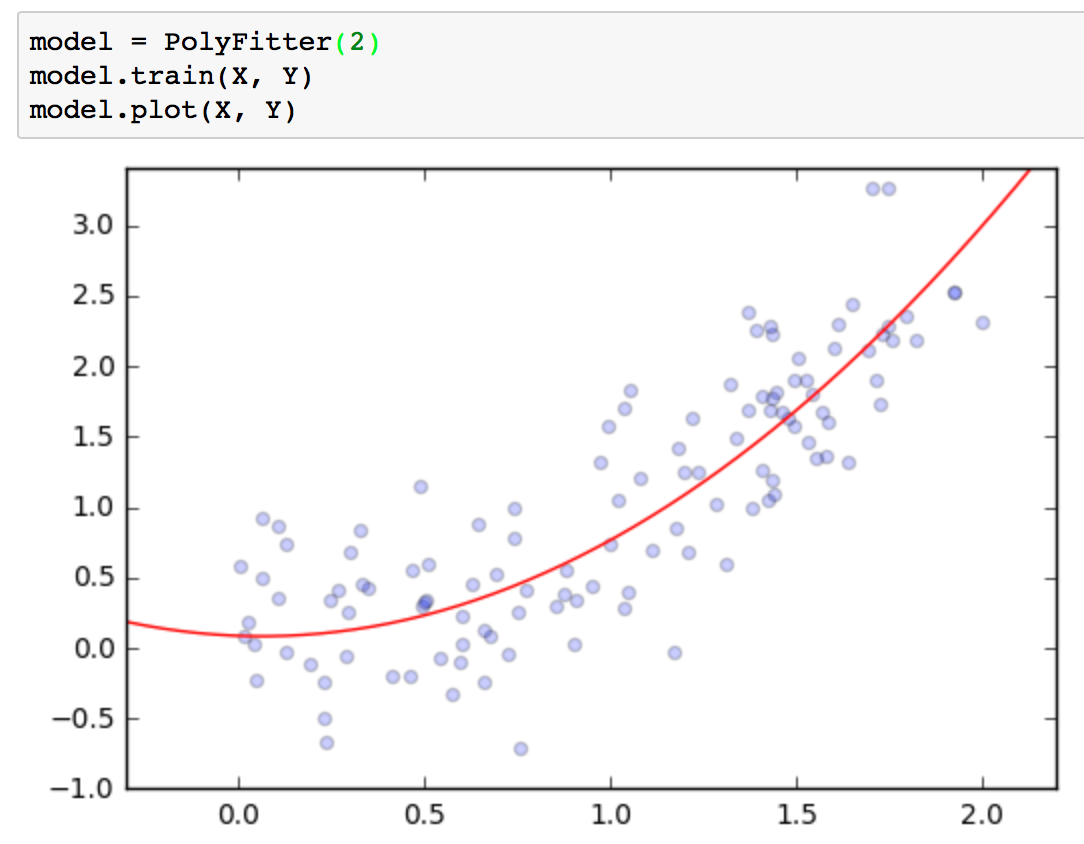
\includegraphics[width=4.0in]{nicefit.png}
\end{center}
\begin{center}
\noindent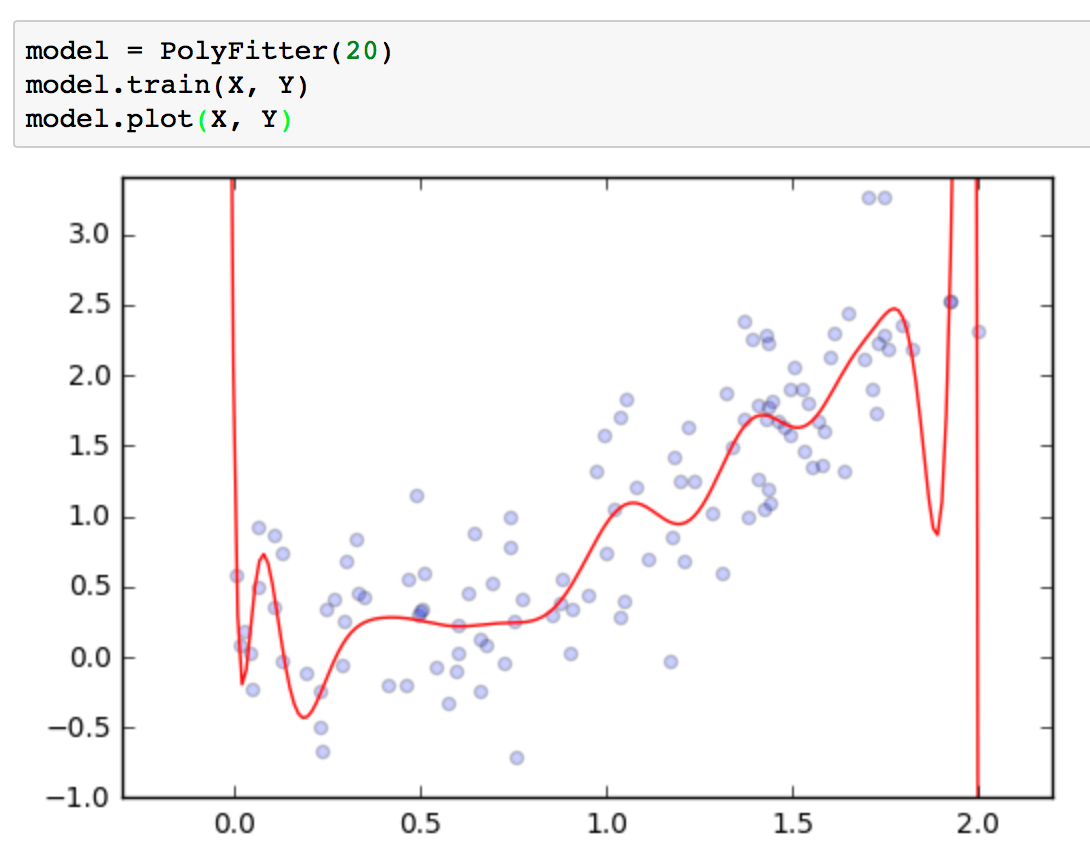
\includegraphics[width=4.0in]{overfit.png}
\end{center}

%\begin{lstlisting}[language=Python]
%from sklearn import linear_model

%class PolyFitter():
    
    %def __init__(self, degree):
        %self.degree = degree
        %self.model = linear_model.LinearRegression()
    
    %def fit(self, X, Y):
        %X_aug = self._augment_input_(X)
        %self.model.fit(X_aug, Y)

    %def predict(self, X):
        %X_aug = self._augment_input_(X)
        %return self.model.predict(X_aug)
    
    %def _augment_input_(self, X):
        %N = X.shape[0]
        %k = self.degree
        %X_aug = np.empty([N,k])
        %X_aug[:,0] = X[:]
        %for i in range(1,k):
            %X_aug[:, i] = X * X_aug[:, i-1]
        %return X_aug
    
    %def plot(self):
        %XX = np.linspace(0,2.2,200)
        %YY = self.predict(XX)
        %plt.scatter(X, Y, alpha=0.2)
        %plt.axis([-1,2,-1,2])
        %plt.plot(XX,YY,"r")
        %plt.show()
        
    %def mean_squared_error(X,Y):
        %# remove pass below and implement mean squared error.
        %# i.e.
        %# you should be using the predict function above
        %pass 
%\end{lstlisting}

\end{itemize}


%The way \code{regr}, a \code{LinearRegression()} object works is that you give it the data to train on. It learns the parameters of the linear model (using least squares method, not gradient descent) based on the training set, and then you can use the \code{predict(XX)} function to compute the value of the function it has learned. Very convenient. 

%The \code{train(X, Y)} function takes an array X of shape \code{(N, k)} where $n$ is  

As you can see, picking a high degree polynomial fits the data much more precisely at certain points. But clearly, this degree 20 aporoximation is not really capturing the essence of this data-set. Your job is:
\begin{itemize}
  \item Write the \code{mean\_squared\_error(X, Y)} function in the class. It should return the average of the square of the difference between the model's predictions (obtained using \code{self.predict(X)}) and the given answers $Y$. This will allow us to see how our model is doing.

  \item Split the data into 75\% training examples and 25\% test examples (You don't need to shuffe the data, just split it). More precisely, from the list \code{data} given to you, make four numpy arrays. $\code{X\_train}$, $\code{Y\_train}$, $\code{X\_test}$ and \code{Y\_test}. The training arrays should contain the $x$ and $y$ coordinates of 75\% of data-points while the test arrays should contain the remaining 25\%. We will use the training pair to train the model, and the test pair to see how our model is doing on data that it has not seen before. This is a standard method for avoiding the mistake of making models that work really well during development, but then work very badly when they see data they have never seen before.
    
  \item For each degree $d = 1,2,3,4,\dots,20$, train a \code{model = PolyFitter(d)} with the data \code{X\_train, Y\_train}, plot what we have using \code{model.plot()} then compute its mean squared error on the training set \code{X\_train, Y\_train}, also compute its mean squared error on the test data-set \code{X\_test, Y\_test}. Plot this `training error' and `test error' over $d=1,\dots,20$.  

\vspace{0.3in}
\begin{center}
\noindent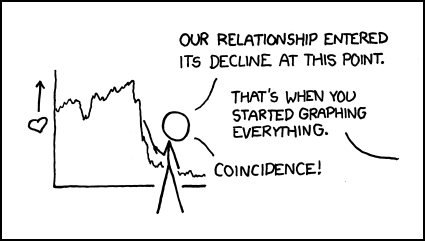
\includegraphics[width=3.5in]{decline.png}

{\tiny Source: XKCD}
\end{center}

You should notice that as the degree increases, the training error goes down a lot, which means that our model is becoming very good at fitting to the training data. But, for the test data, it gets worse and worse. What's the best degree for this data-set?  

\end{itemize}




\subsection*{(Optional) Linear Regression by Gradient Descent} In the lectures, we learned about linear regression, which fits a linear function to a data-set. Download the starter code for this homework from the same page where you downloaded the pdf file. The starter code should come with a file called \code{nba\_data.csv} where we have some data about NBA players. That file should be in the same folder as the starter code notebook.

The first part of the starter code contains code for doing linear regression (using gradient descent) that makes the best possible linear function to guess the weight of an NBA player from the height (weight = a * height +  b ). A few parts of the code are missing: the part that fills the numpy arrays, part that computes the gradient, some of the gradient descent code, \dots). Complete the relevant parts of the code to make it work. Once it works, you should see pictures of our linear approximation at various stages during this `training'. There are more instructions on the starter code notebook. 

(Definitely email me your solution if you do this) Modify the code so that your model approximates the weight as \code{weight = a * height +  b * age + c}. You will need three partial derivatives and update all three variables during gradient descent. Does taking age into account give you a better fit (less total error)? 

%\begin{lstlisting}[language=Python]
%import numpy as np
%import csv
%import matplotlib.pyplot as plt

%# load data
%with open('nba_data.csv', 'r') as f:
    %reader = csv.reader(f)
    %data_list = list(reader)

%# one less because first row of csv file is labels
%N = len(data_list) - 1

%heights = np.zeros(N)
%ages = np.zeros(N)
%weights = np.zeros(N)

%# fill heights ages weights arrays
%for i in range(1, N+1):
    %heights[i-1] = data_list[i][2]
    %ages[i-1] = data_list[i][4]
    %weights[i-1] = data_list[i][3]

%heights_mean = np.mean(heights)
%weights_mean = np.mean(weights)
%ages_mean = np.mean(ages)
    
%heights = heights - heights_mean
%weights = weights - weights_mean
%ages = ages - ages_mean
    
%# this is our model, weight is a linear function of height and age
%def f(a, b, x):
    %return a * x + b

%# total error on the whole data set
%def error_on_data(a,b):
    %return sum([(f(a, b, heights[i]) - weights[i])**2 for i in range(N)]) / N

%# numerical partial derivatives
%h = 0.0000001
%def numdela(fu):
    %return (lambda a,b: (fu(a + h, b) - fu(a, b)) / h)
%def numdelb(fu):
    %return (lambda a,b: (fu(a, b + h) - fu(a, b)) / h)

%eta = 0.005  # learning rate
%num_steps = 601

%a = 0.0
%b = 50.0
%error_amounts = []
%for i in range(num_steps):
    %error_amounts.append(error_on_data(a,b))
    %a = a - eta * numdela(error_on_data)(a,b)
    %b = b - eta * numdelb(error_on_data)(a,b)
    %if i % 40 == 0:
        %plot_data_and_line(a,b)
    
%plot_data_and_line(a,b)
    
%print("final error: ", error_on_data(a,b)) 
%\end{lstlisting}


\end{document}
%%%%%%%%%%%%%%%%%%%%%%%%%%%%%%%%%%%%%%%%%%%%%%%%%%%%%%%%%%%%






